\documentclass[11pt,a4paper]{article}
\usepackage[utf8]{inputenc}
\usepackage[T1]{fontenc}
\usepackage{../tpl} %tdtp
\usepackage{aeguill}
\usepackage{epsfig,graphicx}
\usepackage{subfigure}
\usepackage{eurosym}
\usepackage{enumitem}
\usepackage{hyperref}
\makeatletter


\renewcommand\thesection{Étape \arabic{section} : }
\renewcommand{\theenumi}{Q.\arabic{section}.\arabic{enumi}}

\sorte{TD}
\siglemat{Python et Open data}
\formation{L2 MIASHS}
\titre{Obtention de clés développeur pour l'API Twitter}
\begin{document}

Vous devez préparer un compte Twitter à utiliser pendant la séance. 

\section{Compte Twitter}

Si vous ne disposez pas d'un compte Twitter, vous devrez en créer un. Vous pouvez utiliser votre adresse universitaire.


Si vous possédez déjà un compte Twitter, vous pouvez l'utiliser. 

\section{Numéro de téléphone}
Utiliser les API requiert d'avoir un numéro de téléphone et une adresse mail valides. Vous devez donc vous assurer que votre profil est lié à votre numéro de téléphone. 

Pour ajouter un numéro de téléphone valide, depuis votre profile Twitter, aller dans "Paramètres et confidentialité" puis "Informations du compte".

\begin{center}
    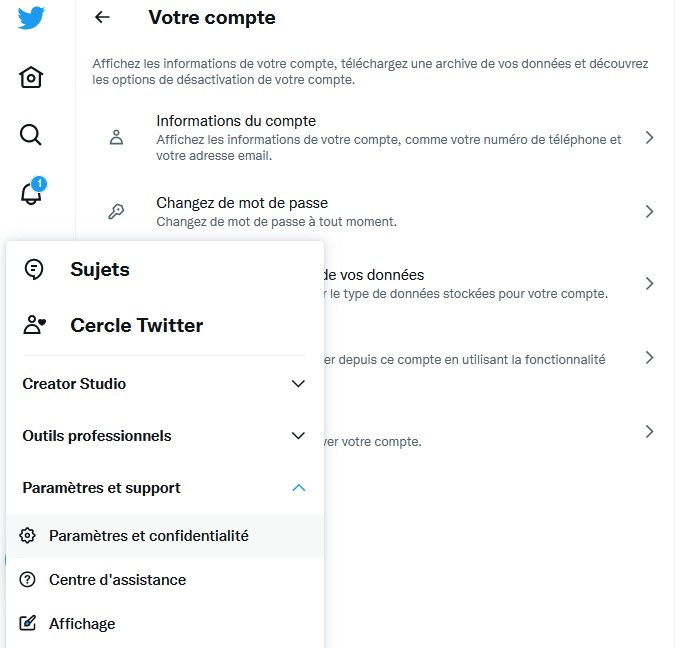
\includegraphics[width=0.4\textwidth]{etapes_cle/step0.jpg}
\end{center}

Note : vous pourrez enlever ultérieurement le numéro de téléphone associé au compte Twitter. 

\newpage
\section{Profil développeur}

Pour pouvoir utiliser l’API Tweepy et récupérer des données sur Twitter, vous devez d'abord créer une application dans l'interface \url{http://apps.twitter.com}.
En allant à cette adresse, vous avez un message indiquant que vous devez activer votre profil développeur, comme ci-dessous. 
\begin{center}
    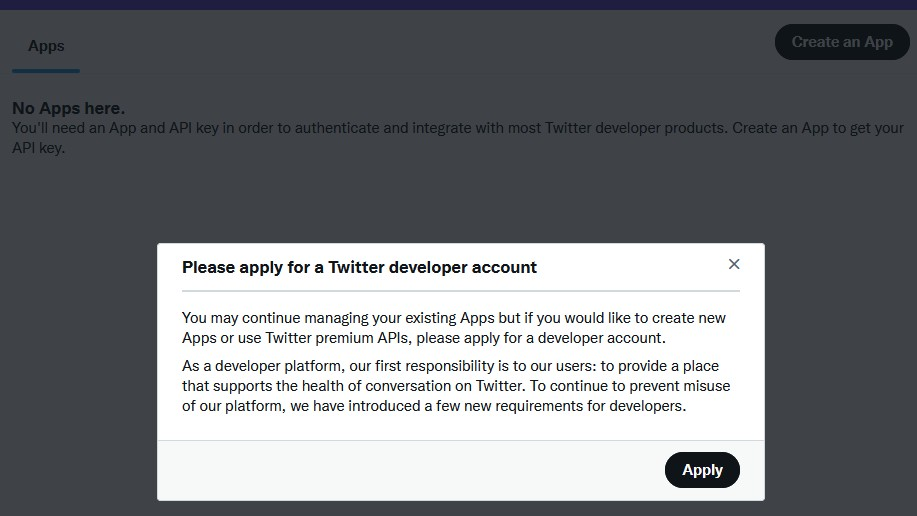
\includegraphics[width=0.5\textwidth]{etapes_cle/step1.jpg}
\end{center}

Lancer la création d'un compte développeur. Vous pouvez renseigner les champs en indiquant que vous êtes étudiant, comme ci-dessous (nous configurons sur l'exemple le profile de Christiane, \emph{chris\_suspecte}). 

\begin{center}
    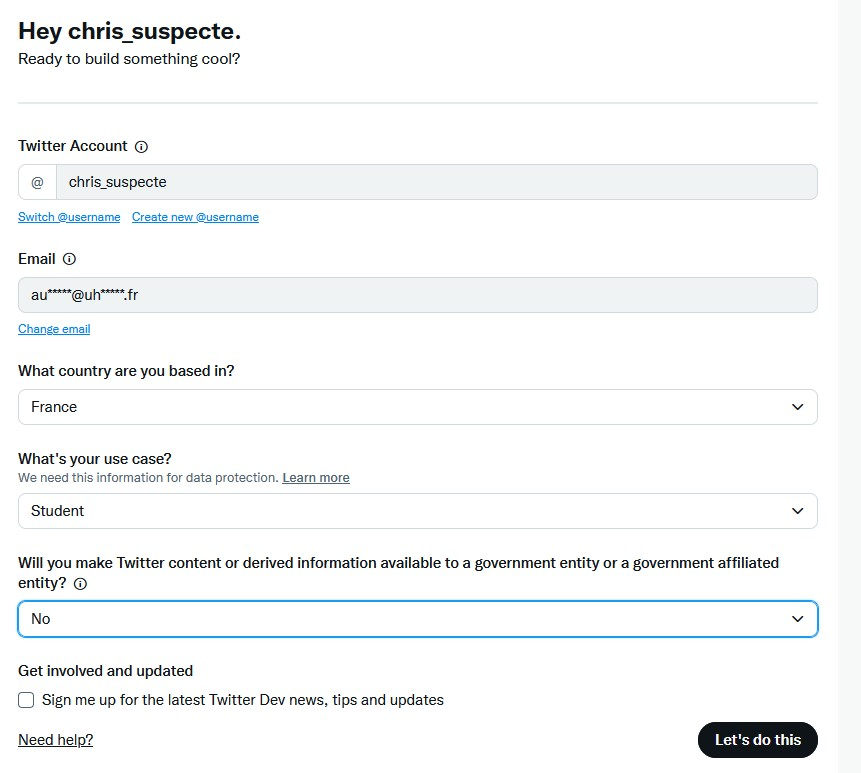
\includegraphics[width=0.6\textwidth]{etapes_cle/step2.jpg}
\end{center}

Vous devez ensuite accepter les conditions, et valider votre email. 
\newpage
\section{Application}

Lorsque votre profil développeur est validé, on vous propose de créer une application. Renseignez un nom de projet comme ci-dessous\dots
\begin{center}
    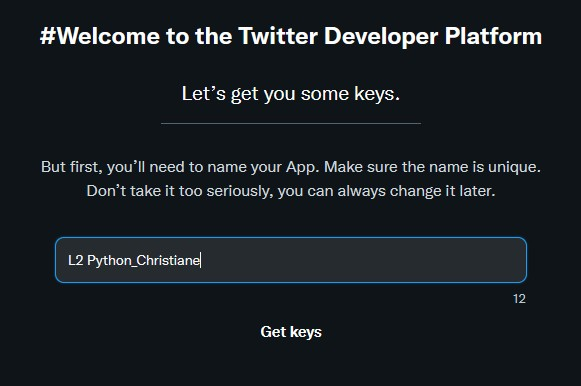
\includegraphics[width=0.4\textwidth]{etapes_cle/step3.jpg}
\end{center}
puis demandez les clés. 

Notez soigneusement, et de manière confidentielle, \textbf{les deux clés CONSUMER} : API key et API Key Secret.

\section{Droits en écriture du projet}
Après avoir noté vos clés, accéder au Dashboard, et plus précisément à votre \emph{App} dans \emph{Projects \& Apps}.
Sur cette page, dans la section \emph{User authentication settings}, cliquez sur \emph{Set up}, puis modifiez les permissions pour demander les droits en lecture et écriture avec le projet. 

Cela nécessite d'indiquer l'adresse mail d'un site web, indiquez l'adresse de l'université :  \url{http://www.univ-rennes2.fr}.

\begin{center}
    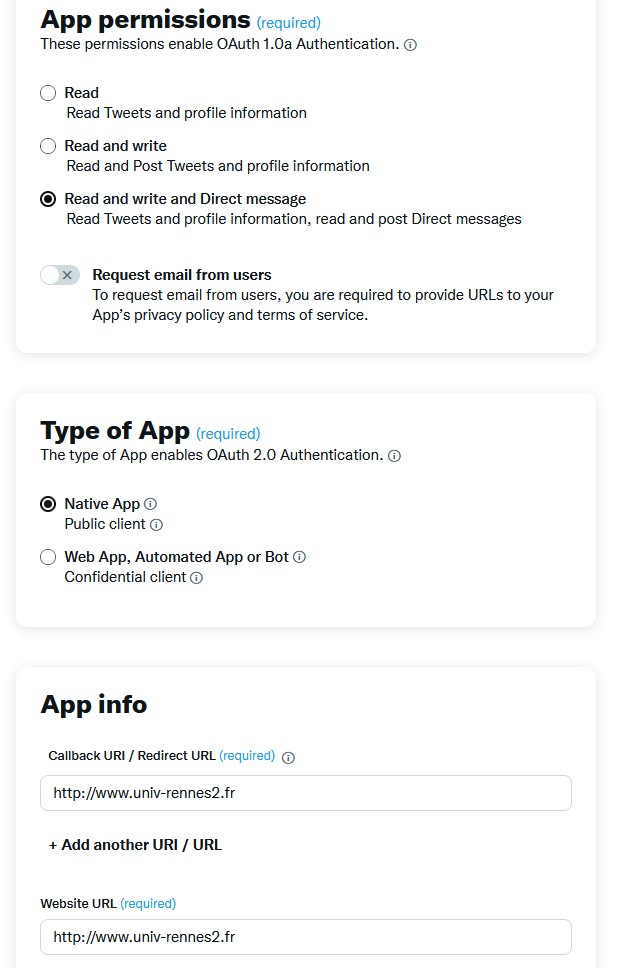
\includegraphics[width=0.4\textwidth]{etapes_cle/step5.jpg}
\end{center}


\section{Token d'accès}

Il faut maintenant générer les token d'accès en cliquant sur "Generate" pour les Access Token and Secret, comme ci-dessous. 
\begin{center}
    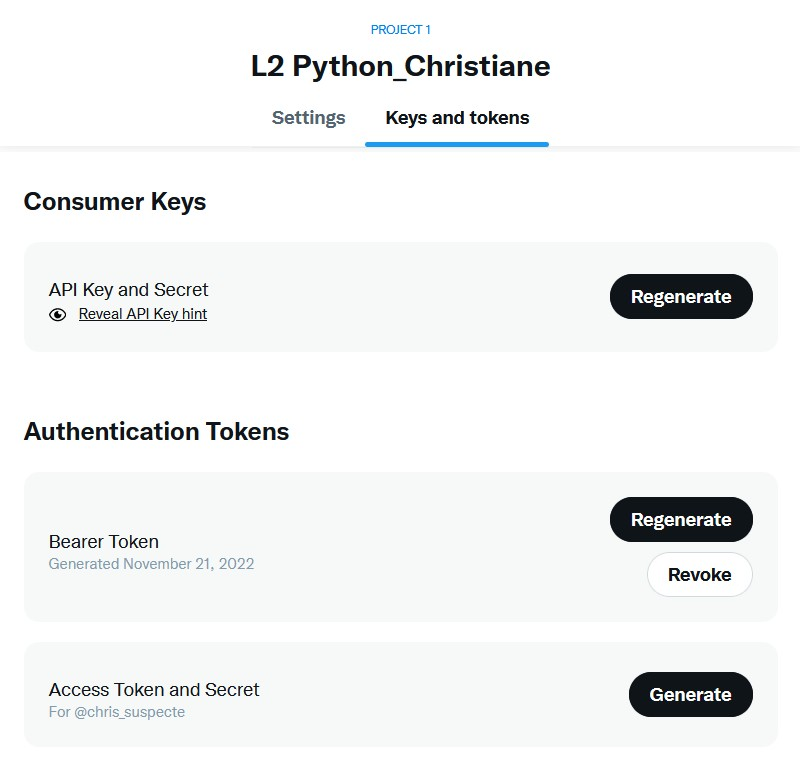
\includegraphics[width=0.4\textwidth]{etapes_cle/step4.jpg}
\end{center}
Notez soigneusement, et de manière confidentielle, \textbf{les deux clés ACCESS TOKEN } : Access Token et Access Token Secret.







\section{Accès elevated}
Par défaut, le compte développeur créé a un niveau \emph{essential}. Pour disposer des fonctionnalités nécessaires au TD, nous souhaitons utiliser un profil \emph{elevated}.

Dans le portail développeur, chercher à gauche Products, puis Twitter API-v2. Demander à souscrire un niveau Elevated. 

\begin{center}
    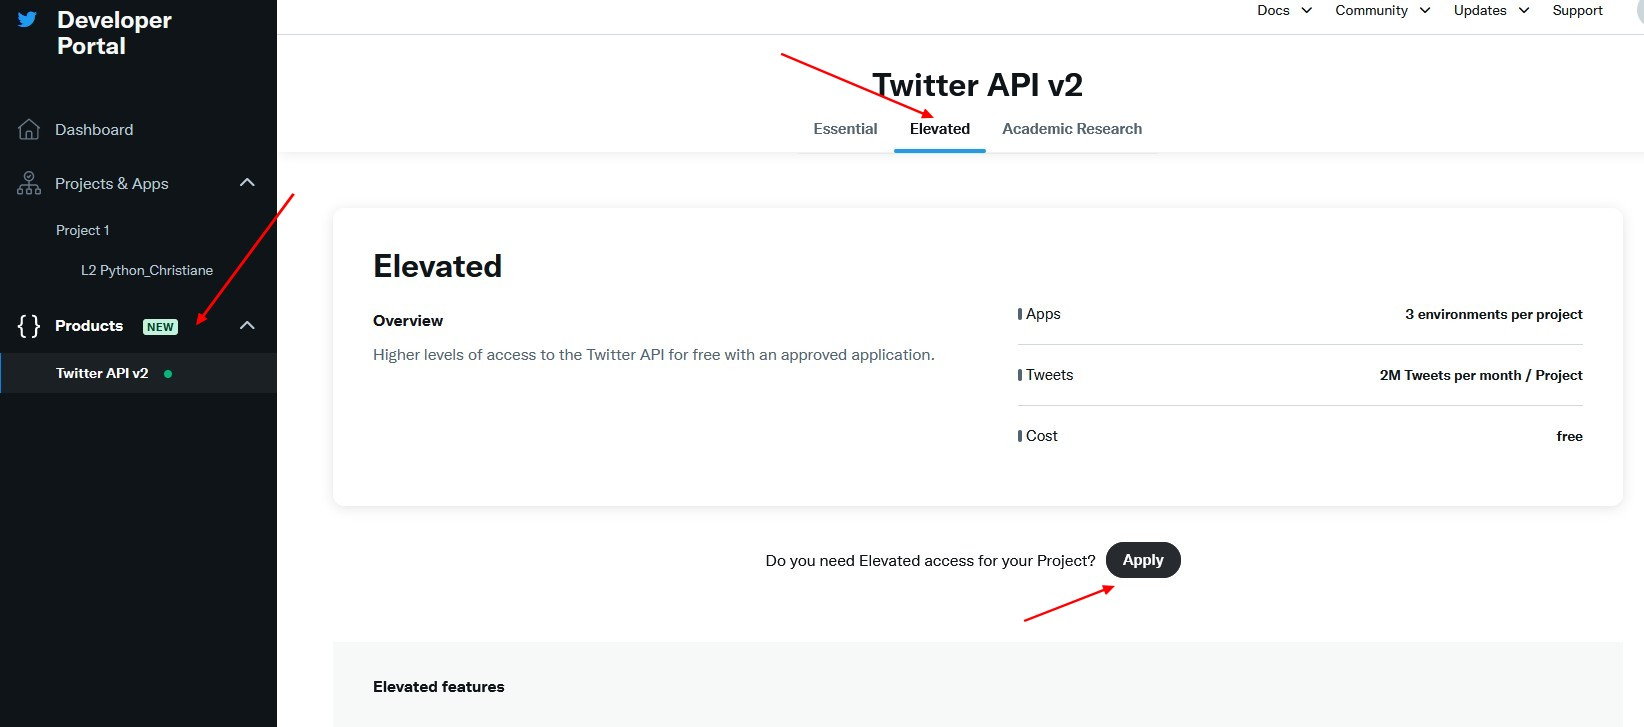
\includegraphics[width=0.8\textwidth]{etapes_cle/step6.jpg}
\end{center}

La souscription demande plusieurs étapes de validations. Il faut notamment indiquer quelles sont vos intentions avec l'API. Nous vous proposons de coller le texte suivant : 

\emph{
I will use Tweeter API jointly with the tweepy Python module in a course at the bachelor level. The goal is to learn how to use APIs in Python programs. I have no plan to analyze tweets in any way, I will just play with the tweepy module to understand what it allows.
I will not tweet, retweet or like content except for demo purposes. There is no end-user solution planned.
}

et de cocher No pour les différents items. 

\begin{center}
    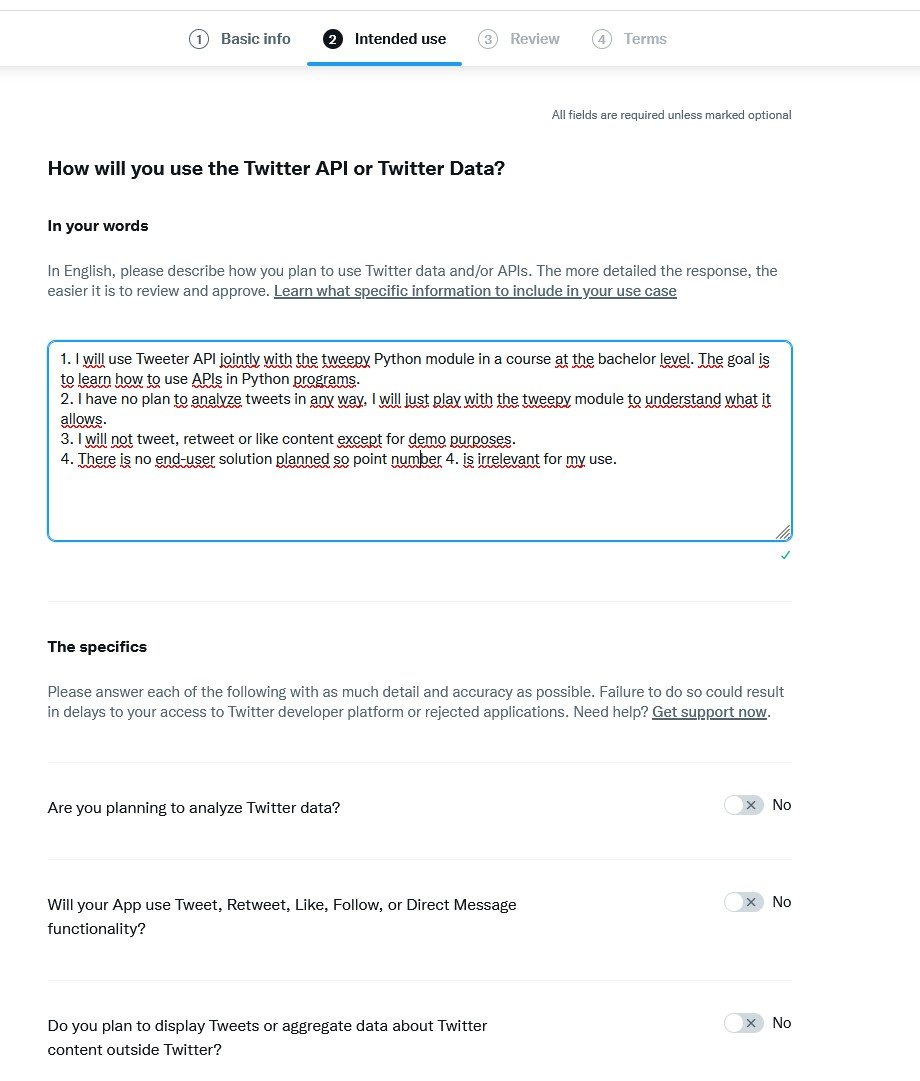
\includegraphics[width=0.6\textwidth]{etapes_cle/step7.jpg}
\end{center}

\section{C'est prêt !}
Au final, vous disposez donc de 4 clés que vous pouvez écrire dans un fichier :
\begin{verbatim}
"CONSUMER_KEY":"xxxx"
"CONSUMER_KEY_SECRET":"xxxx",
"ACCESS_TOKEN":"xxxx",
"ACCESS_TOKEN_SECRET":"xxxx"
\end{verbatim}


\end{document}
